\documentclass[SE,lsstdraft,authoryear,toc]{lsstdoc}
% GENERATED FILE -- edit this in the Makefile
\newcommand{\lsstDocType}{PSTN}
\newcommand{\lsstDocNum}{057}
\newcommand{\vcsRevision}{4a7a175-dirty}
\newcommand{\vcsDate}{2026-06-03}



\defcitealias{PSTN-056}{pstn-056}
\defcitealias{LPM-17}{SRD}

\newcommand{\todo}[1]{{\color{red} #1}}
\newcommand{\new}[1]{{\color{blue} #1}}
\newcommand{\incomplete}[1]{{\color{blue} [PROVISIONAL RECOMMENDATION ] #1}}
\newcommand{\pz}{{Photo-$z$}}

\newcommand{\opsim}{\texttt{OpSim}}
\newcommand{\baseline}[1]{{\texttt{baseline\_v#1}}}
% Package imports go here.
\usepackage{placeins}
%\usepackage[printwatermark]{xwatermark}
%\usepackage{xcolor}
%\usepackage{graphicx}
%\newwatermark[allpages,color=red!50,angle=45,scale=3,xpos=0,ypos=0]{DRAFT}
\usepackage{overpic}
% Package imports go here.

% Local commands go here.

%If you want glossaries
%\input{aglossary.tex}
%\makeglossaries

\title{Survey Cadence Optimization Committee’s Survey Start Recommendations}

% This can write metadata into the PDF.
% Update keywords and author information as necessary.
\hypersetup{
    pdftitle={Survey Cadence Optimization Committee’s Survey Start Recommendations},
    pdfauthor={Federica B. Bianco and the SCOC},
    pdfkeywords={}
}
\author{%
The Rubin Observatory Survey Cadence Optimization Committee
}

% Optional subtitle
% \setDocSubtitle{A subtitle}

\input{authors}

\setDocRef{PSTN-057}
\setDocUpstreamLocation{\url{https://github.com/lsst-pst/pstn-057}}

\date{\vcsDate}

% Optional: name of the document's curator
% \setDocCurator{The Curator of this Document}

\setDocAbstract{%
A recommendation for adjustments to the initial LSST survey strategy is delivered to the Observatory Director. These adjustments respond to improved knowledge and understanding of the system performance and completeness of science verification activities at the start of LSST.
}

% Change history defined here.
% Order: oldest first.
% Fields: VERSION, DATE, DESCRIPTION, OWNER NAME.
% See LPM-51 for version number policy.
\setDocChangeRecord{%
  \addtohist{1}{YYYY-MM-DD}{Unreleased.}{Bianco}
}


\begin{document}

% Create the title page.
\maketitle

With the Vera C. Rubin Observatory (Rubin) now having completed the transition from Construction to Operations, and on the eve of the start of the Legacy Survey of Space and Time \citep[LSST][]{LPM-17},  Rubin remains committed to continuing to optimize the LSST survey strategy to maximize the scientific return on the four LSST Science Pillars and beyond. 

The Survey Cadence Optimization Committee (hereafter SCOC\footnote{\url{https://rubinobservatory.org/for-scientists/committees-teams/scoc}}) is a Rubin standing committee tasked with soliciting, collecting, and aggregating community input on the expected science performance of proposed LSST survey strategies and optimizing it to make strategy recommendations to the Rubin Director, who makes the final decision on implementation (see \citealt{Bianco_2022}). 

We now have an updated understanding of system performance, which indicates a decrease in expected survey time of about $10\%$ once accounting for more realistic expectations on engineering and downtime, and telescope performance. A plan has also been developed to start LSST while Rubin continues to improve both the delivered image quality and effective survey speed during the first 1-2 years of the survey, leading to additional engineering time and decreased image quality, both improving through Year 1 (Y1). Finally, while a plan to collect incremental sky templates during Y1 was designed based on the assumption that the desired template depth and image quality could be achieved with $\sim3$ exposures of sufficient quality (measured generally as seeing \todo{$\mathrm{FWHM}\leq 1.4$ and
transparency $\phi \geq 0.75$}), a deeper understanding of the process of template construction reveals that templates constructed with $<5$ images would be highly incomplete due to chip gaps and masking, requiring modification to the incremental template construction strategy \citep{rtn-011}. Within this framework, we recommend updates to the most recent SCOC recommendation in \citealt{PSTN-056}  for the observing planned to take place at the start of LSST and during Y1 of the survey.

\section{Recommended changes to the observing strategy}\label{sec:recommendation}
The proposed survey design for Y1 is to follow the \texttt{baseline\_v5.0}, which is an implementation of PSTN-056 (which itself builds on earlier SCOC recommendations \citealt{pstn-053} and  \citealt{pstn-055})  for footprint (PSTN-056 recommendation vi and xxiii), filter balance (i, ii, viii, ix, xx), rolling (iii, and v), including not starting rolling in Y1 (xxi), special surveys (DDF, PSTN-056 recommendations xvi and xviii, ToO, x-xiv, Twilight microsurvey, xxii), observing in single exposures rather than ``snaps'' (PSTN-056 recommendations xv) and cadence,  with the following changes:

\begin{enumerate}
\item We introduce a ``template-tier'' observing mode that is activated when sky conditions (atmospheric seeing) are conducive to the collection of good PSF images that can be used to build sky templates. This observing mode attempts to collect five images in each filter and relaxes the constraints on image pairs implemented in the main survey (but see point two) to accelerate the production of templates over the LSST footprint (as recommended in PSTN-056 and described in \citealt{rtn-011} to support early science).

\item The template tier collects images in pairs (primarily in different filters), but the pairs are spaced by median $\mathrm{t_{pair gap}}=20$ minutes, slightly less than the median time gap for image pairs collected in main survey mode. Bluer bands ($u$ and $g$) may be acquired in same-filter pairs, to more tightly pack these visits into available good-seeing dark time. Observing in pairs enables tracking of solar system objects even in the absence of templates, and provides colors for transients and variables observed in the images, although the color will only be measured retroactively once the templates are available. Overall, this observing mode preserves the efficiency gains of the template tiers while enabling additional science outcomes. 

\item Since depth is not the limiting factor that requires the use of $>3$ exposure for templates, reduced exposure time for each image may enable the construction of templates that are sufficiently complete and deep to enable DIA processing and DIA-based science, while increasing the efficiency of constructing the incremental templates. The SCOC favorably reviews the scientific impact of collecting $20$ ($28$) seconds exposures for $grizy$ ($u$) template exposures in the template tier observing mode. However, a feasibility study is pending, to ensure the shorter exposure (1) does not impact data processing negatively, (2) truly leads to a higher efficiency in delivering templates (\eg are the image cycles correspondingly faster and the image quality as good based on AOS performance) (3) does not negatively affect system calibration. Particular attention should be paid to the image quality expectations in $u$ band, where 28 seconds is close to the readout limit. Retaining the standard $38$~sec exposure time in $u$ while reducing exposure time in other filters may be the optimal solution, and we expect the feasibility study to deliver an answer. Pending the outcomes of this feasibility study, the SCOC recommends the collection of templates with shorter exposures as described above.

\item Translational and rotational dithering between visits within a night in the Deep Drilling Fields (DDFs) are added to translational and rotational dithering between nights following the current recommendations from Data Management (DM), although the SCOC continues to invite studies of options to reduce dithering to maximize the DDF stack depth and highest-cadence region footprint (PSTN-056 recommendation xvii).

\item \new{Finally, in PSTN-056 and \texttt{baseline\_v5.0} we introduce a specific DDF observing strategy (PSTN-056 recommendation xviii) dubbed ``ocean'' that observes DDFs in either ``deep'' or ``ultradeep'' seasons.  Each field receives one ultradeep season (except COSMOS, which receives three), with long sequences of visits within a night. The deep seasons have shorter sequences (typically two or three visits in each filter). Both the deep and ultradeep seasons have high cadence, with nightly observations in alternating filters (so typically two-night cadence in any given filter).} 
\end{enumerate}

At this stage, the SCOC is not recommending any additional changes to the observing strategy. However, as system performance continues to evolve, we remain responsive to changes and opportunities, we continue to solicit and collect community input, and further recommendations may follow as needed throughout the course of Y1.

\section{Baseline 5.3}\label{sec:opsims}

The \texttt{baseline\_v5.3} simulation includes our current best estimates for the system on-sky uptime, slew performance, and engineering time needs, which are still evolving. The simulation’s start date is broadly estimated to be consistent with the start date for LSST, but should not be considered as a forecast or a commitment to the official start date of the survey.\footnote{The start of LSST is proposed by Rubin’s Start of LSST Board to the Rubin Observatory Director, who will make the final decision after consulting with the Rubin Management Board and funding agencies.}

The addition of more maintenance time in every year (46 weeks total instead of 20), additional engineering test time (one night every month plus two half-nights a week for the first six months), and a more realistic fault time per night result in a reduction of the overall number of visits on-sky of about 10\% compared to the \texttt{baseline\_v5.0} simulation upon which the Phase 3 SCOC recommendation is based (PSTN-056). This 10\% reduction is seen in each year (the reader is reminded that previous simulations starting with \texttt{OpSim v3.6}, already included significant additional downtime within Y1).

In more detail, in \opsim\ \texttt{v5.3} we increased the planned maintenance from 2 weeks/year to 3 weeks/year + 8 weeks in years 4 and 8; added 2 half nights of engineering observations per week for the first 6 months and 1 night every 25 days later (including calibration); kept the \texttt{v5.0} 19 weeks of unplanned downtime in years 2-10 and extended this into year one for a total of 21 weeks of unplanned downtime; and modified short intervals of unplanned downtime early in the survey, which was modeled starting at $\sim25\%$ and progressively reducing to $\sim3\%$ over year one in \texttt{v5.0}, now is $\sim20\%$ to $\sim5\%$ ramping down over three years. 


The TMA performance is modeled as 20\% max slew speed and 3-second settle time. This performance is undergoing optimization, with some known avenues for improvement. This estimate is expected to be a slightly optimistic at the start of LSST and pessimistic later on. However, we conservatively maintain this performance throughout the survey as the timeline for improvements is still uncertain.


Beyond these updates, the \texttt{baseline\_v5.3.0} observing strategy implements the SCOC recommendations described in \autoref{sec:recommendation}.

%A template tier aims to obtain “template-quality images” in pairs when the sky conditions are favorable. 

 \autoref{fig:performance} shows the performance of the proposed \texttt{baseline\_v5.3} for a core set of selected science-driven metrics (the extended set of metrics used by the SCOC for its deliberation includes hundreds), compared to earlier simulations of the LSST survey starting with \texttt{baseline\_v5.0}, which implements the recommendation in PSTN-056.  \texttt{baseline\_v5.1.2} introduces the template tier observing mode (described in \autoref{sec:recommendation}, \#1), and is otherwise consistent with \texttt{baseline\_v5.0}; \texttt{comp\_v5.3} assumes the same sky availability as \texttt{baseline\_v5.0}, but implements the template tier in pairs in different filters (\autoref{sec:recommendation}, \#2), and DDF observing schema (\autoref{sec:recommendation}, \#4 \& 5) as \texttt{baseline\_v5.3}. This simulation is made available to demonstrate that the specific strategy choices recommended in this note are not \emph{per sè} causing any scientific losses, rather they generate gains in most metrics, and the lower performance of \texttt{baseline\_v5.3} as compared to earlier baselines is in fact entirely driven by lower sky availability. Finally, \texttt{20s fast templates\_v5.3} implements the shorter exposure time for the template tier observations (\autoref{sec:recommendation}, \#3).

\autoref{fig:nvisits} shows the coverage of the LSST footprint as a function of number of visits. SRD \todo{minimum} requirements are marked.

\todo{LYNNE DO WE WANT A BETTER FIGURE HERE?? I would like a figure with baseline 3,4,5.0 5.1 comp 5.3  baseline 5.3 and baseline 5.3 with 20 sec exposures. -LJ: I added the figure I think you have asked for. }



\begin{figure}
    \centering
    %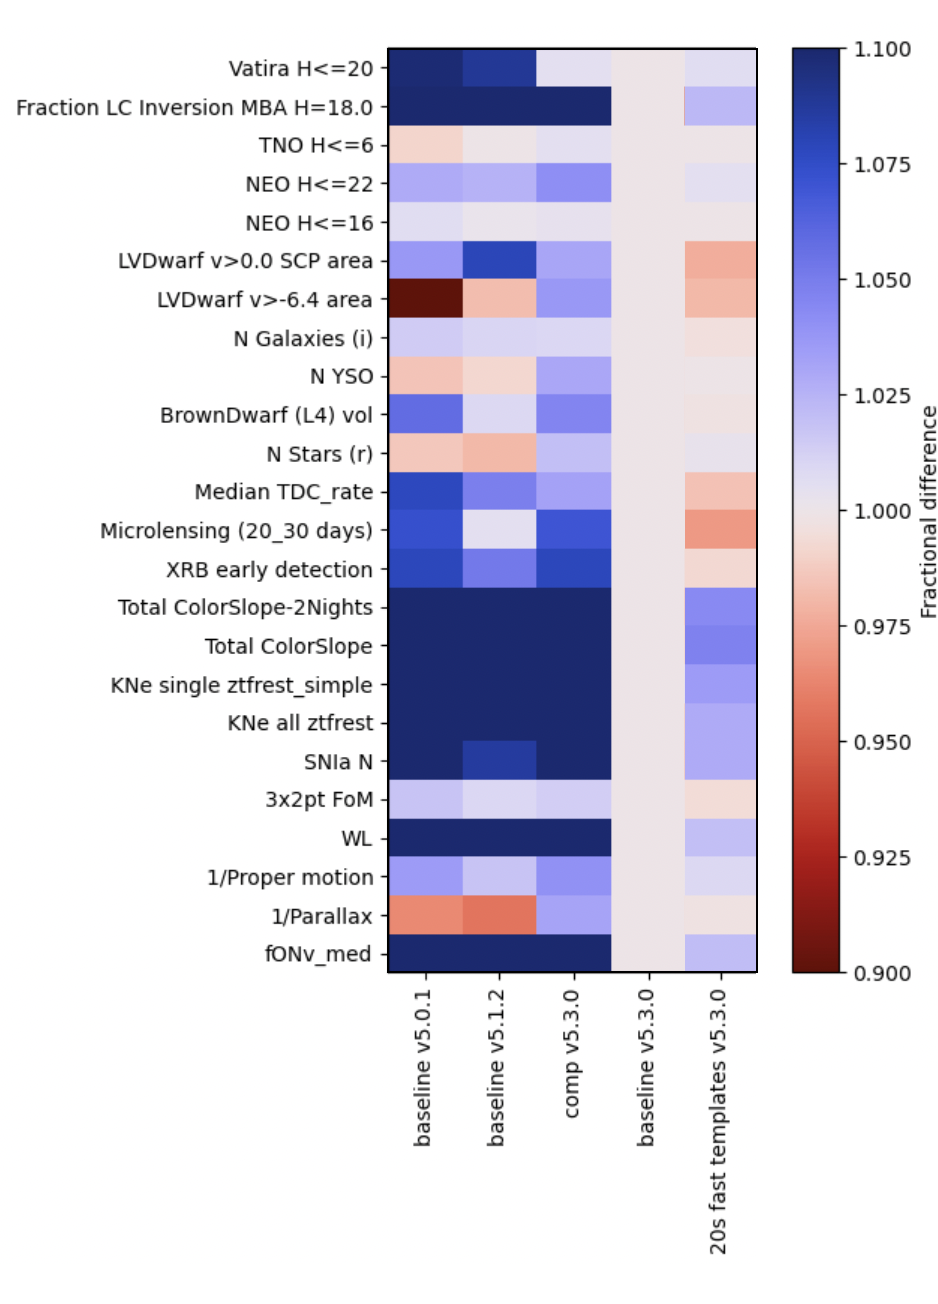
\includegraphics[width=0.5\linewidth]{figures/opsimperformance.png}
    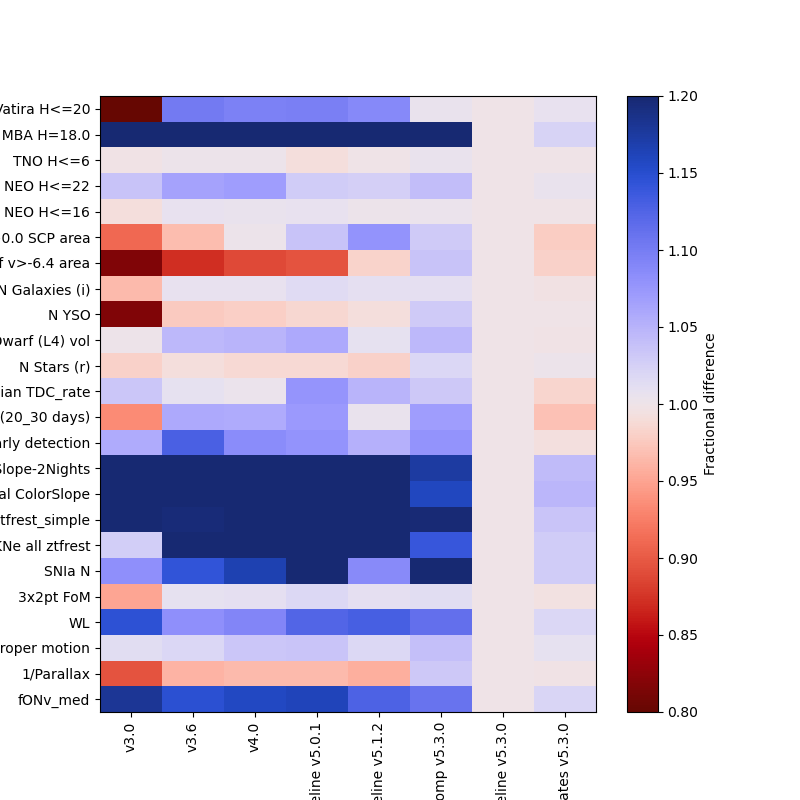
\includegraphics[width=0.5\linewidth]{figures/scoc_grid.png}
    \caption{Performance of the presently recommended strategy compared to previous baselines. The plot compares the performance of selected metrics (labeled along the $y$ axis) across baseline simulations (along the $x$ axis) from \texttt{baseline\_v5.0.1} through \texttt{baseline\_v5.3} and its short-template exposure implementation (see \autoref{sec:recommendation}). The details of each \opsim\ are included in \autoref{sec:opsims}. In this plot, \texttt{baseline\_v5.3} is selected as the reference (\ie its performance is set to 1 for all metrics) and the performances of all other \opsim s are shown relative to that. Blue colors indicate a positive metric value, \ie an improvement. 
    Red colors indicate a performance drop with respect to the reference \opsim . The reduced sky time availability drives the performance loss in \texttt{baseline\_v5.3}. Note the stretch of the colormap: in this heatmap, the darker blues indicate a ≥10\% improvement, and the darkest reds a ≥10\% drop. Several metrics, in particular the ones measuring time domain phenomena (\texttt{color-slope} metrics that generally measure our ability to identify anomalies, kilonovae metrics, \texttt{KNe}, and the supernova \texttt{SNIa N} metric), solar system lightcurves characterization metrics (\texttt{Fraction LC Inversion MBA H=18.0}), but also weak lensing (\texttt{WL}) and the number of visits \texttt{fONv\_med}, are impacted by 10\% or more and are saturated in this plot.   The introduction of shorter template exposures (\texttt{20s fast templates\_v5.3}) has a modest impact on most metrics and an overall positive impact on most time domain related metrics, recovering some performance for most metrics that had been most impacted by the reduced sky availability. However, none of these metrics include a concept of template readiness, so the advantage of the earlier availability of templates and of increased template completeness in Y1 is not represented in this plot.}
    \label{fig:performance}
\end{figure}

\begin{figure}
    \centering
    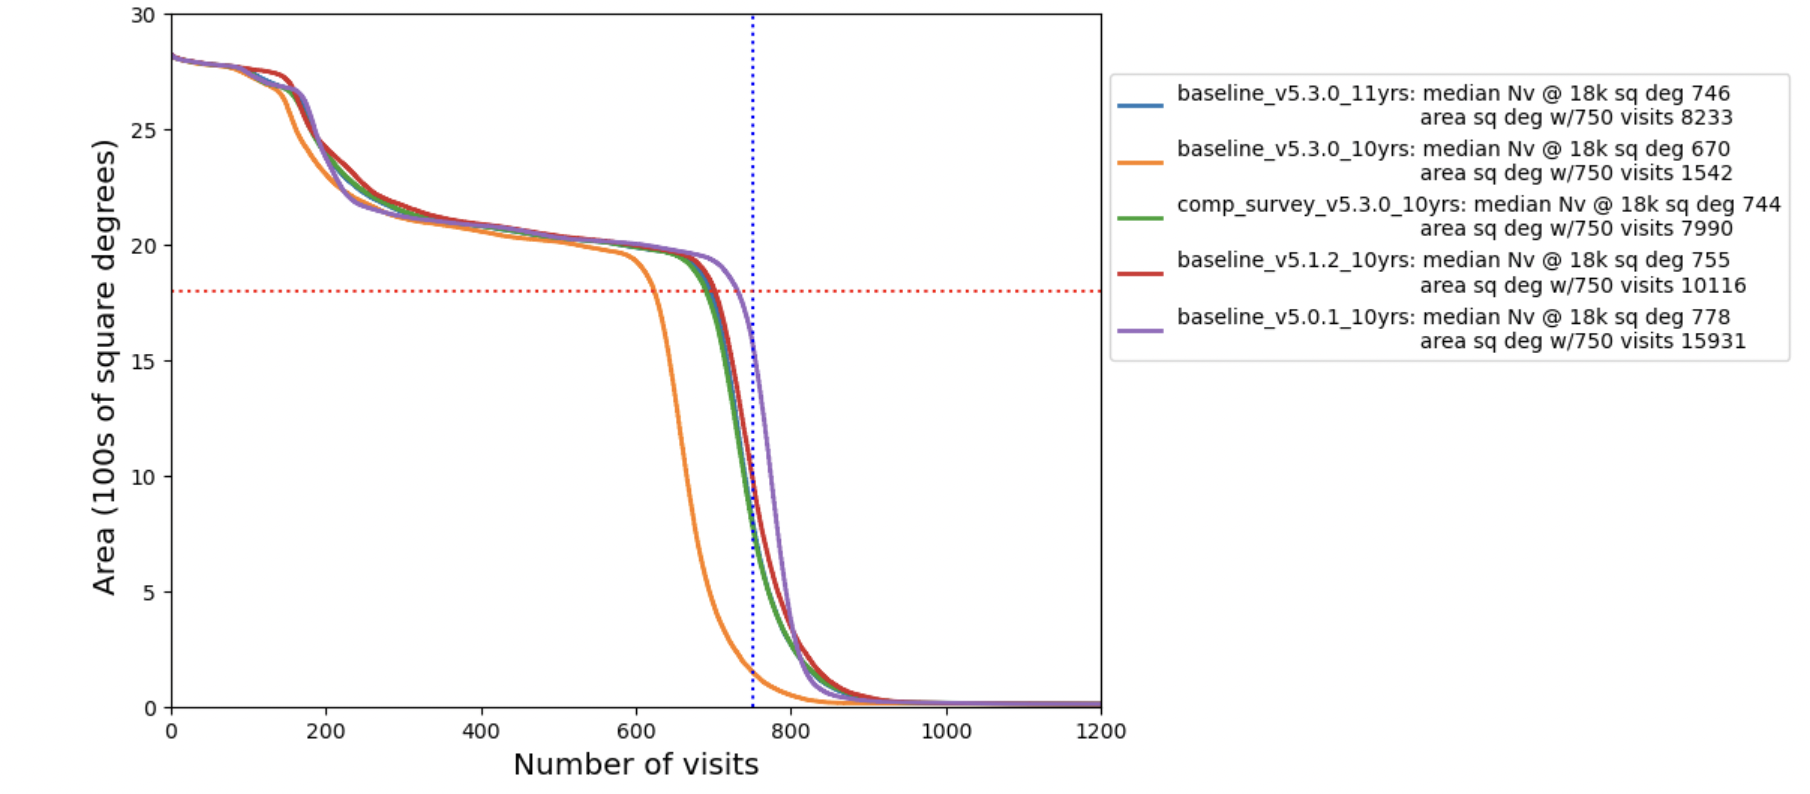
\includegraphics[width=0.9\linewidth]{figures/nvisits.png}
    \caption{The LSST footprint area as a function of the number of visits at the end of the LSST. Vertical and horizontal dotted lines represent the minimum and design LSST requirements (LPM-17) for the number of visits and area, respectively. A selected subset of \opsim  s as described in section \autoref{sec:opsims} is included. \todo{Lynne I forget why there is a drop from 5.0 to 5.1 .. (answered in slack) }. }
    \label{fig:nvisits}
\end{figure}

\appendix

\section{Acknowledgements}

This material is based upon work supported in part by the National Science Foundation through Cooperative Agreements AST-1258333 and AST-2241526 and Cooperative Support Agreements AST-1202910 and AST-2211468 managed by the Association of Universities for Research in Astronomy (AURA), and the Department of Energy under Contract No.\ DE-AC02-76SF00515 with the SLAC National Accelerator Laboratory managed by Stanford University.
Additional Rubin Observatory funding comes from private donations, grants to universities, and in-kind support from LSST-DA Institutional Members.

% Include all the relevant bib files.
% https://lsst-texmf.lsst.io/lsstdoc.html#bibliographies
\section{References} \label{sec:bib}
\renewcommand{\refname}{} % Suppress default Bibliography section
\bibliography{local,lsst,lsst-dm,refs_ads,refs,books}

% Make sure lsst-texmf/bin/generateAcronyms.py is in your path
\section{Acronyms} \label{sec:acronyms}
\addtocounter{table}{-1}
\begin{longtable}{p{0.145\textwidth}p{0.8\textwidth}}\hline
\textbf{Acronym} & \textbf{Description}  \\\hline

AST & NSF Division of Astronomical Sciences \\\hline
AURA & Association of Universities for Research in Astronomy \\\hline
DE-AC02 & Department of Energy contract number prefix \\\hline
LSST & Legacy Survey of Space and Time \\\hline
LSST-DA & LSST Discovery Alliance \\\hline
PSTN & Project Science Technical Note \\\hline
SLAC & SLAC National Accelerator Laboratory \\\hline
\end{longtable}

% If you want glossary uncomment below -- comment out the two lines above
%\printglossaries





\end{document}
